\documentclass[]{article}
\usepackage{graphicx}
\usepackage{hyperref}
\usepackage{amsmath}
\usepackage{caption}
\usepackage{subcaption}
\usepackage{ngerman}

%opening
\title{Balmer Series}
\author{Gunther T\"urk, Jonas Lehnen}

\begin{document}

\maketitle
\begin{abstract}


\end{abstract}

\tableofcontents

\newpage
\section{Theorie}
\subsection{Bohr Modell}
Der klassische Ansatz ein Atom zu beschreiben ist ungenügend. Normalerweise würde man ein durchgängiges Spektrum an Strahlung erwarten, da der Abstand zwischen Kern und Elektron zunächst nicht beschränkt ist. Das Gegenteil wird jedoch gemessen. Ebenso sollte von einer bewegten Ladung Strahlung emittiert werden, dies geschieht im Atom jedoch nur wenn sich der Abstand verkleinert. Dies bewegte Bohr 1913 dazu seine Postulate zu formulieren. Darin beschreibt er, dass das Elektron den Kern umkreist und durch die elektrostatische Kraft auf seiner Umlaufbahn gehalten wird ohne dabei Strahlung auszusenden. Diese Bahnen werden durch ihren Drehimpuls $l = pr = n\hbar$ beschrieben. Hier bei beschreibt $n$ die Ordnung der Bahn, auch Hauptquantenzahl genannt. Zuletzt entspricht die Energie des emittierten bzw. absorbierten Photons dem Energieunterschied des Elektrons auf verschiedenen Umlaufbahnen $ \hbar \omega = E_2 - E_1$. 

Generell erhält man aus der Behandlung der Schrödingergleichung dieselbe Energie für verschiedenen $n$, welche auch aus der Gleichsetzung von Coulomb- und Zentripetalkraft folgt. $R_\infty$ wird auch Rydbergkonstante genannt. 
\[E_n = -\frac{1}{2} m_0 c^2 \alpha^2 \frac{Z^2}{n^2} = -13.6eV \cdot \frac{Z^2}{n^2} \: ; \: \alpha = \frac{e^2}{4\pi\epsilon_0 \hbar c} = \frac{1}{137}\]

\[\Delta E = R_\infty \left(\frac{1}{n^2} - \frac{1}{m^2} \right)  = -13.6eV \cdot \left(\frac{1}{n^2} - \frac{1}{m^2} \right)\]

Dadurch können wir nun die Photonenenergie bestimmen, wenn ein Elektron seinen Bahn ändert. Im folgenden sowie bereits in der zweiten Gleichung behandeln wir das Wasserstoff Atom mit $Z=1$.Hierbei wird in verschiedene Serien unterschieden, je nachdem in welche das Elektron landet, nach Photon-Emission. Jede Serie wurde nach Entdecker benannt. Die ultravioletten Spektrallinien der Lyman (Ly) Serie $Ly_\alpha \:,\: Ly_\beta \:,\: Ly_\gamma \:,\: ...$ besitzt als Grundniveau den Zustand $n=1$. Analog wurden auch die infraroten Serien Brackett (B) $n=4$ und Paschen (Pa) $n=3$, sowie die sichtbare Balmer (H) Serie $n=2$ entdeckt. 
Die lateinische Nomenklatur beschreibt von wie vielen Niveaus oberhalb, auch states genannt, das Elektron auf das Endniveau gefallen ist. Die Anzahl wird mit den Buchstaben gleichgesetzt. So hei"st der \"Ubergang $5 \rightarrow 2$ auch $B_\gamma$.

\subsection{Ebert Monochromator}
Um nun die das Licht eines Elements analysieren zu können mpüssen wir die spektrallinien auffächern. Hier im Experiment wird dies mit einer Form des Ebert Monochromators umgesetzt. Dabei handelt es sich um um zwei  Spalte durch die das Licht ein- und ausfallen kann. Während dem Durchgang wird der Lichtstrahl zwischen zwei Reflexionen an einem Hohlspiegel auch an einem Gitter umgelenkt. Dieses Gitter ist nun drehbar und der Winkel $\delta$ in \ref{fig:Monochromator} bezeichnet die Verstellung bezüglich der parallel Lichtstrahlen. 

\begin{figure}[!h]
\centering
\begin{subfigure}{0.55\textwidth}
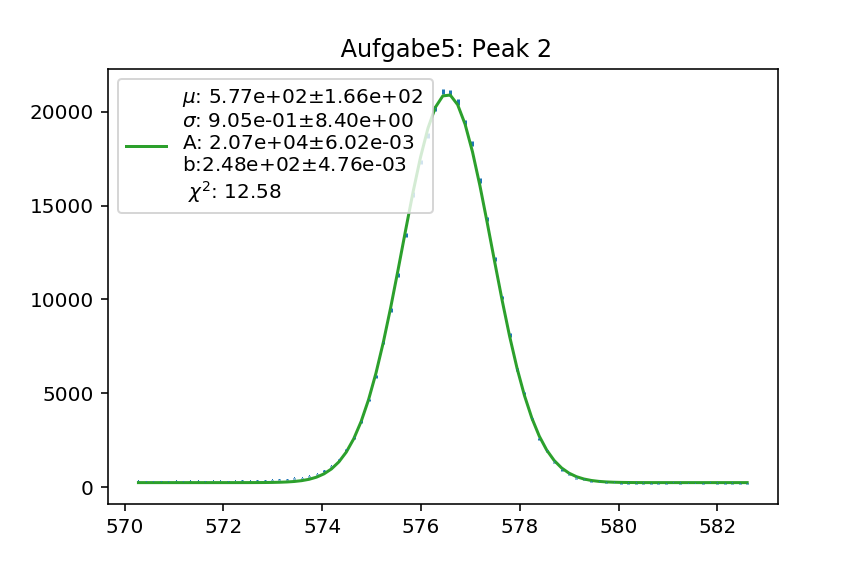
\includegraphics[width=\linewidth]{Plots/1.png}
\end{subfigure}
\begin{subfigure}[c]{0.4\linewidth}
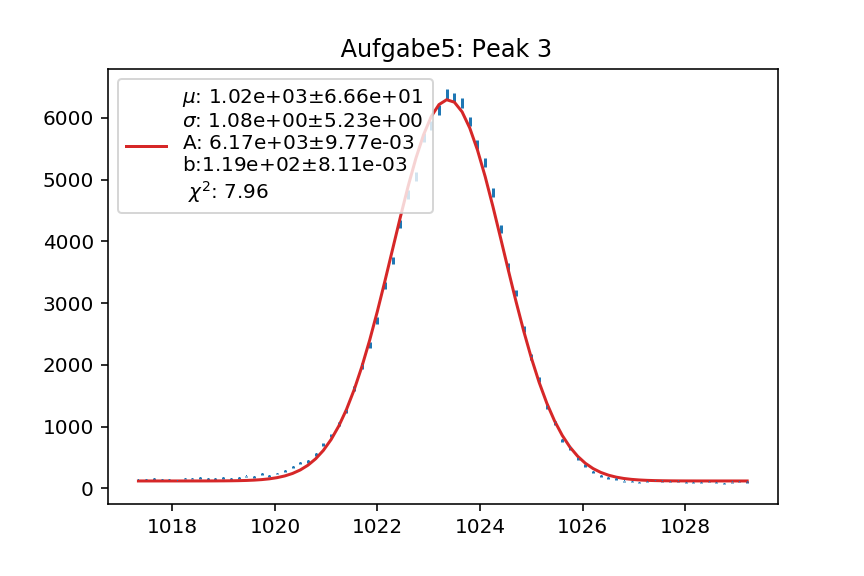
\includegraphics[width=\linewidth]{Plots/2.png}
\end{subfigure}
\caption{Schematische Darstellung eines Ebert Monochromators. Grafiken wurden dem zum Experiment mitgegebenen Skript (SS 2006) entnommen. }
\label{fig:Monochromator}
\end{figure}



\newpage
\section{Experiment}
\subsection{Setup}
Hier im Expermient wird ein Ebert Monochromator benutzt. 

\section{Anhang}


\newpage
\begin{thebibliography}{}


\end{thebibliography}
\end{document}

